\newpage
\begin{center}
    \section{L'entreprise SMOI, une expérience unique}
\end{center}

\subsection{Un ressentis contraster}
% 1, 2 et 5

Lors de mon stage j'ai pu faire les frais d'un environnement de travail difficile, avec énormément de bruit d'un niveau sonore très élevé (normal pour un atelier de construction métallique) engendrant des difficultés de compréhension de ce qu'on essayais de me dire, mais il y avait aussi une forte exposition au soleil, augmentant d'autant plus la pénibilité des tâches à réaliser.\newline
Malgré cet environnement de travail difficile, l'ambiance de travail en elle-même au sein de l'entreprise est douce, chaleureuse et amicale. Ainsi même en cas de soucis ou de difficulté lié à la timidité ou en étant nouveau donc comme cela était mon cas, l'ambiance est incroyablement chaleureuse et celle-ci permet alors de tisser des liens et d'avoir un très bon relationnel. J'ai donc malgré ma timidité et difficulté à communiquer avec les autres immédiatement été rassuré.\newline

Cette ambiance de travail se reflétait également avec de bonnes conditions de sécurité avec des règles très strictes. Ce stage m'a alors permis de beaucoup apprendre sur comment était réalisé les charpentes des bâtiments, les étapes à suivre, leur but mais aussi le fonctionnement des machines. Et c'est cette partie même qui m'a le plus plu dans mon stage, avoir la possibilité d'en apprendre plus sur un sujet et de découvrir le fonctionnement des machines ainsi que des méthodes de fabrication et avoir ainsi l'expérience d'une application directe de la théorie apprise en classe.\newline
Mes activités me permettent ainsi d'avoir une connaissance plus large sur le domaine de la fabrication, les procédés utilisés, leur but et le fonctionnement des machines, provoquant alors un fort sentiment de satisfaction en regardant le travail qu'on a réalisé terminer et se rendre ainsi compte de tout ce qu'on peut vraiment faire soit même avec de la matière première et les bon outils.\newline

Dans l'entreprise j'ai réalisé des tâches de fraisage, découpe, gravure et polissage, j'ai donc en résumer réaliser les tâches de la préparation intermédiaire des matière première avant l'assemblage et la peinture de celle-ci. Des tâches qui dans cette société ne sont pas automatisées puisque chaque élément est fait sur mesure en fonction de critères des clients en particulier et non pas pour la grande distribution.\newline
J'occupais alors une place importante dans la chaîne de fabrication puisqu'étant placé à l'étape juste avant l'assemblage des pièces.



\subsection{un stage présentant des difficulté inattendu}
% 3 et 4

Avant d'effectuer mon stage j'avais quelque appréhension concernant le côté relationnel qui n'est pas mon point fort. J'ai ainsi rencontré comme je le craignais des difficulter à m'adapter à l'ambiance qui régnait ainsi qu'à développer le côté relationnelle. Cependant j'ai également dû faire face à un difficultés que je ne pensais pas arrivé qui était les difficultés de compréhension du au vocabulaire précis utiliser que je pensais connaître suffisamment avant d'avoir réaliser mon stage.\par
J'ai donc pour palier à ces difficultés, dans un premier temps au niveau relationnelle, forcé la conversation en essayant d'en apprendre plus sur les autres membre de l'atelier mais également en essayant d'en comprendre plus sur le fonctionnement des machine ainsi que sur la raison et l'utiliser de certain procédé et méthode de fabrication. En ce qui concerne les problème de compréhension je n'ai cependant pu totalement m'en débarrasser, puisque je ne pouvais pas voir l'entièreté du vocabulaire de l'atelier juste sur une ou deux mission réalisé, j'ai du apprendre tout au long de mon stage du nouveau vocabulaire au fil des jours et palier de manque de compréhension par des demande d'explication.



\subsection{une entreprise en pleine innovation}
% cf qcm annexe 2 + DU

J'ai pu constater lors de mon stage que la société SMOI était en constante évolution avec la présence d'une innovation qui est l'agrandissement de l'atelier et la mise en place d'un raille de transport permettant de transporter les matière première et celle de transition d'un bout à l'autre de l'atelier pour leur transformation, une innovation permettant d'accélérer et facilité la production (donc étant bénéfique pour les ouvriers) de part une plus grande mobilité et un plus grand espace de travail.\ref{fig:innovation}\newline
Une entreprise innovante mais qui tout de même à mon avis, après en avoir discuté avec le gérant, pourrait s'améliorer sur un autres point, ici plus accès sur la sécurité au travail avec le \acrshort{DU}* qui même s'il est revu chaque année en fonction des nouvelles missions et/ou du nouveau matériel à disposition, ne présente pas vraiment de suivi de la bonne réalisation des normes et précautions mis en place que cela soit par un service interne liée à la sécurité du travail ou par des prestataires externes.\footnote{cf annexe 1} \newline

Je suggérerais donc en voie d'une amélioration de leur système et politique de sécurité au travail, en vue notamment de cette innovation (agrandissement de l'atelier) qui va entraîner la naissance de nombreux autres risque pour la sécurité des travailleur, de soit mettre en place un secteur dédié à la rédaction de ce Document Unique ainsi qu'à sa communication et au contrôle de sa bonne suivit en interne ou encore de faire appel à un prestataire extérieur spécialisé dans ce domaine de la sécurité au travail afin de contrôler l'application de ces mesure et d'avoir un retour concret sur celle-ci pour les modification futur du DU.
\begin{figure}[h!]
    \centering
    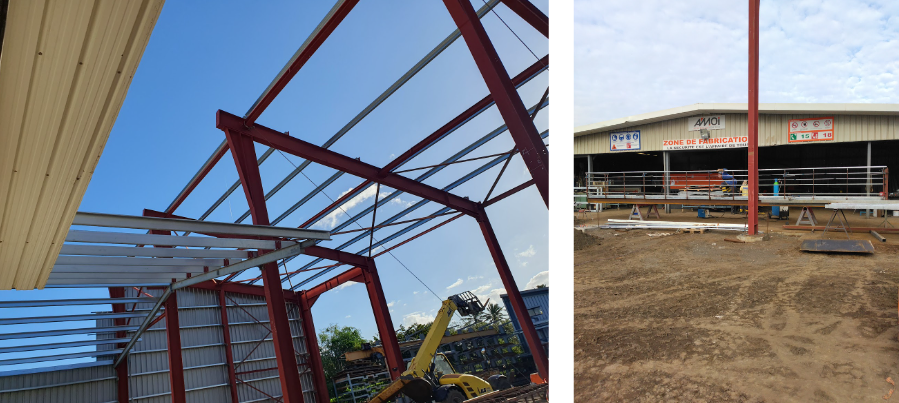
\includegraphics[width=1\linewidth]{figures/innovation.png}
    \caption{photo du projet d'innovation en cours}
    \label{fig:innovation}
\end{figure}



\subsubsection{Conclusion}
%mini conclusion et résumé des info de la partie

Pour conclure cette partie, la société SMOI est très accueillante, et présente de nombreux points positifs quant à la sécurité et sur l'innovation et sont amélioration, malgré la présence de quelque point négatif notamment au niveau du suivi du respect des mesure du DU. J'ai alors rencontré quelques difficultés qui se sont rapidement résolues par une implication relationnelle de ma part. Me permettant ici de mieux appréhender l'importance de chaque main, du relationnel mais aussi les réflexions autour de l'innovation et de la sécurité dans le monde de l'entreprise.